\section{Pengujian}
\label{sec:pengujian}


Tujuan dari pengujian ialah untuk memastikan apakah seluruh kebutuhan fungsional dan non-fungsional dari sistem telah terpenuhi.
Untuk pengujian kebutuhan fungsional, pengujian dibagi menjadi dua bagian yaitu pengujian yang dilakukan per komponen lalu dilanjutkan dengan pengujian sistem. Setiap skenario pengujian dijelaskan tujuannya, skenario yang dilakukan, dan hasil pengujian yang didapatkan. Skenario pengujian akan memiliki ID dengan awalan P diikuti dengan dua angka. Seluruh pemetaan pengujian terdapat pada lampiran \ref{chapter:tabel-pengujian}

\subsection{Batasan Pengujian}
\label{subsec:batasan-pengujian}
Berikut adalah batasan yang ditetapkan dalam melakukan pengujian \textit{sistem remote deployment}.

\begin{enumerate}
  \item Pengujian dilakukan di tiga kluster yang berbeda
        \begin{enumerate}
          \item Kubernetes lokal \textit{cluster}
          \item \textit{Google Cloud Platform (GCP) Compute Engine} Kubernetes \textit{cluster}
          \item RaspberryPi Cluster
        \end{enumerate}
  \item Setiap \textit{cluster} memiliki jumlah node yang sama yaitu 2.
  \item \textit{Cluster} dibuat dengan distribusi kubernetes k3s.
  \item Sistem \textit{remote deployment} dijalankan pada komputer lokal yang memilki spesifikasi yang telah dijelaskan pada bagian \ref{sec:lingkungan-implementasi}.
  \item Untuk beberapa fungsionalitas admin digunakan \textit{HTTP Client} yaitu Postman untuk membuat \textit{request} kepada \textit{service}
  \item Cluster sudah tersedia dan siap diakses.
  \item Setiap \textit{request} memiliki header X-Api-Key.
  \item Setiap \textit{request} yang mengarah ke /admin-api/ memiliki \textit{header} berupa X-Admin-API-Key.
  \item \textit{Database} pada bagian "deployment images" sudah terisi sebagian untuk memudahkan proses pengujian.
\end{enumerate}

\subsection{Persiapan Pengujian}
Pada proses pengujian, terdapat tiga lingkungan pengujian yang digunakan untuk menguji sistem \textit{remote deployment}. Ketiga lingkungan tersebut yaitu kubernetes \textit{cluster} lokal, kubernetes \textit{cluster} yang terdapat di \textit{Cloud (GCP)}, serta \textit{cluster} pada RaspberryPi. Ketiga \textit{cluster} ini memiliki jumlah node yang berbeda sesuai dengan penjelasan pada \ref{subsec:batasan-pengujian}.

\subsubsection{Kubernetes Lokal}
Untuk pengujian pada kubernetes lokal, dilakukan pembuatan \textit{cluster} dengan kakas kind untuk membuat cluster yang bernama \textit{testing-cluster-two-nodes} yang memiliki 2 node. Konfigurasi pembuatan sama seperti konfigurasi pada bagian \ref{subsec:persiapan-kubernetes-cluster} hanya saja jumlah nodes yang digunakan yaitu 2.
Karena nodes berjumlah dua maka terdapat 1 \textit{master nodes} dan 1 \textit{slave} node pada \textit{cluster}. Konfigurasi pembuatan cluster dapat dilihat pada gambar \ref{fig:kubernetes-lokal-config-testing}.

\begin{figure}[htbp]
    \centering
    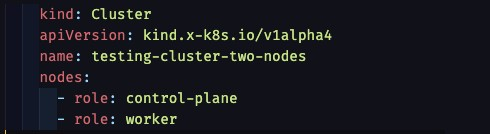
\includegraphics[width=1\textwidth]{resources/chapter-4/pengujian/kubernetes-lokal-config.jpg}
    \caption{Konfigurasi Pembuatan \textit{Kubernetes Testing Cluster} Dengan Kakas \textit{Kind}}
    \label{fig:kubernetes-lokal-config-testing}
\end{figure}

Setelah itu jalankan perintah "kind create cluster --config testing-cluster.yaml" untuk membuat \textit{cluster} pada \textit{docker}. Hasil dari perintahh ini yaitu tercipta dua buah \textit{container} pada \textit{docker} yang memiliki peran \textit{master} dan \textit{slave} seperti pada gambar \ref{fig:kubernetes-lokal-config-testing-result}.

\begin{figure}[htbp]
    \centering
    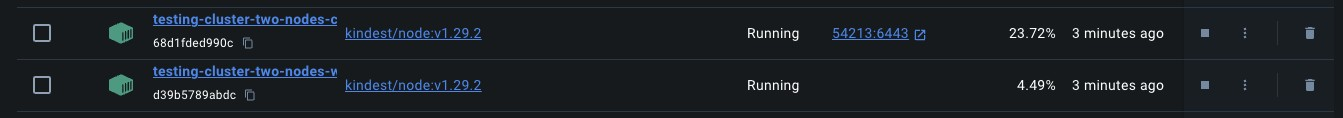
\includegraphics[width=1\textwidth]{resources/chapter-4/pengujian/kubernetes-lokal-config-result.jpg}
    \caption{Hasil \textit{Kubernetes Testing Cluster} pada \textit{Docker}}
    \label{fig:kubernetes-lokal-config-testing-result}
\end{figure}

\subsubsection{Kubernetes GCP}
\label{subsubsec:kubernetes-gcp}
Pada lingkungan ini dibuat dua buah \textit{compute engine (virtual machine)} pada \textit{GCP}. Masing masing dari \textit{virtual machine} berperan sebagai kubernetes \textit{cluster} yang bernama \textit{prod-cluster-example}.

\begin{enumerate}
    \item Buat dua \textit{virtual machine} pada \textit{compute engine GCP} dengan spesifikasi berikut. Hasil pembuatan \textit{virtual machine} dapat dilihat pada lampiran \ref{fig:hasil-pembuatan-virtual-machine-gcp}
          \begin{enumerate}
              \item Ubuntu 24.04
              \item 2GB Memory
              \item 10GB Storage Persistent Disk
              \item 0.5 - 2Vcpu (1 shared core)
              \item Region Asia southeast2-c
          \end{enumerate}
    \item Membuat \textit{Firewall Rule} Untuk membuka port yang digunakan oleh Kubernetes. Untuk daftar opsi setiap port yang dibuka dapat dilihat pada lampiran \ref{fig:daftar-kegunaan-port}. Untuk hasil pembuatan firewall dapat dilihat pada lampiran \ref{fig:hasil-firewall-rule-pada-gcp}
    \item Konfigurasi \textit{gare-test-kubernetes-server} sebagai master nodes. Konfigurasi dilakukan dengan cara mengunduh instalasi dari k3s dengan perintah seperti pada lampiran \ref{fig:instalasi-master-node-gcp}.
    \item Konfigurasi virutal machine lainnya yaitu \textit{gare-test-kubernetes-server-node} sebagai \textit{worker node}. Untuk meregistrasi \textit{node} ke dalam \textit{cluster} perlu adanya autentikasi untuk memasitikan hanya \textit{node} yang benar yang boleh masuk ke dalam \textit{cluster}. K3s memiliki token generator yang dapat digunakan untuk mencegah akses yang tidak diinginkan, registrasi token dapat dilihat pada lampiran \ref{fig:pengambilan-token-registrasi-cluster}. Token tersebut digunakan untuk meregistrasi \textit{node} ini ke \textit{master} dengan \textit{public ip} node tersebut. Ilustrasi dapat dilihat pada lampiran \ref{fig:instalasi-worker-node-gcp}.
    \item Ambil konfigurasi \textit{cluster} di \textit{master node} dan pindahkan ke lokasi \textit{server berjalan} untuk meregistrasi \textit{cluster} ke dalam sistem. Setelah melakukan kelima langkah ini \textit{cluster} sudah terintegrasi dengan sistem. Ilustrasi pemindahan konfigurasi dapat dilihat pada lampiran \ref{fig:konfigurasi-cluster-master-node-gcp} dan \ref{fig:proses-pemindahan-konfigurasi-master-gcp}.
\end{enumerate}

\subsubsection{Kubernetes RaspberryPi}
Pada lingkungan ini dibuat cluster dengan dua nodes pada RaspberryPi. Cluster yang dibuat bernama cluster-raspi yang memiliki spesifikasi hardware RaspberryPi berikut.

\begin{enumerate}
    \item Master node menggunakan Raspberry Pi 3 Model B Rev 1.2 dengan 1GB RAM dan 4 CPU @ 1.2GHz dengan hostname masterpi. Informasi lebih lengkap dapat dilihat pada lampiran \ref{fig:hostname-raspi-master-nodes} dan \ref{fig:spesifikasi-raspi-master-nodes}
    \item Worker node menggunakan Raspberry Pi 2 Model B Rev 1.1 dengan 1GB RAM dan 4 CPU @ 900MHz dengan hostname raspberrypi. Informasi lebih lengkap dapat dilihat pada lampiran \ref{fig:hostname-raspi-worker-nodes} dan \ref{fig:spesifikasi-raspi-worker-nodes}
\end{enumerate}

Berikut merupakan tata cara pembuatan cluster kubernetes pada \textit{RaspberryPi}. Diasumsikan \textit{device} \textit{RaspberryPi} sudah terhubung ke dalam jaringan yang sama sehingga tidak perlu \textit{port forwarding} / \textit{public ip}.

\begin{enumerate}
    \item Konfigurasi \textit{hostname masterpi} sebagai master nodes. Perlu dilakukan konfigurasi tambahan untuk menambahkan cgroups pada raspberrypi karena secara default opsi ini \textit{disabled}. cgroups merupakan kepanjangan dari \textit{Control Groups} yang berfungsi sebagai \textit{resource management} pada linux dan digunakan dalam proses kontainerisasi. Selanjutnya mirip serperti konfigurasi pada bagian \ref{subsubsec:kubernetes-gcp}, perlu mengunduh instalasi dari k3s dengan perintah seperti pada lampiran \ref{fig:instalasi-master-raspi-nodes}.
    \item Konfigurasi \textit{node} lainnya yaitu \textit{hostname raspberrypi} sebagai \textit{worker node}. Untuk meregistrasi \textit{node} ke dalam \textit{cluster} perlu adanya autentikasi untuk memasitikan hanya \textit{node} yang benar yang boleh masuk ke dalam \textit{cluster}. K3s memiliki token generator yang dapat digunakan untuk mencegah akses yang tidak diinginkan, registrasi token dapat dilihat pada lampiran \ref{fig:raspi-master-gen-token}. Token tersebut digunakan untuk meregistrasi \textit{node} ini ke \textit{master} dengan \textit{ip local} node master. Ilustrasi dapat dilihat pada lampiran \ref{fig:instalasi-worker-raspi-node}.
    \item Ambil konfigurasi \textit{cluster} di \textit{master node} dan pindahkan ke lokasi \textit{server berjalan} untuk meregistrasi \textit{cluster} ke dalam sistem. Setelah melakukan langkah ini \textit{cluster} sudah terintegrasi dengan sistem. Ilustrasi pemindahan konfigurasi dapat dilihat pada lampiran \ref{fig:raspi-kube-config} dan \ref{fig:raspi-add-kubeconfig}.
\end{enumerate}

\subsection{Pengujian Komponen}
Pengujian di level komponen memastikan bahwa seluruh fungsionalitas yang tidak melibatkan servis eksternal di dalam komponen bekerja dengan baik. Pengujian ini dibagi menjadi beberapa bagian sesuai dengan domain yang telah dijelaskan pada bagian \ref{subsec:implementasi-service}. Pada masing masing domain terdapat tabel yang memetakan hubungan antara kebutuhan fungsional serta pengujian yang bersesuaian. Pengujian dilakukan menggunakan lingkungan lokal dengan nama cluster "kind-testing-cluster-two-nodes"

\subsubsection{Fungsionalitas pada Domain Company}

Pengujian dengan ID P01 dilakukan dengan skenario yaitu admin berhasil membuat \textit{company} baru dengan nama \textit{cluster} yang tersedia pada sistem. Tersedia artinya konfigurasi kubernetes \textit{cluster} terdapat pada kubernetes \textit{config server}. Daftar \textit{cluster name} yang tersedia dapat dilihat pada lampiran \ref{fig:list-cluster-tersedia}. Admin membuat request dengan Postman kepada \textit{server} dengan request seperti berikut.

\begin{enumerate}
  \item Mengisi \textit{field name} dengan nilai "new company"
  \item Mengisi \textit{field cluster\textunderscore name} dengan nilai "kind-testing-cluster-two-nodes"
\end{enumerate}

\textit{Request} dibuat dengan membuat request menggunakan Postman pada url /admin-api/v1/companies dengan metode POST. \textit{Request dan Response} dapat dilihat pada lampiran \ref{fig:pengujian-p01}

Pengujian dengan ID P02 dilakukan dengan skenario yaitu admin tidak berhasil membuat \textit{company} karena nama cluster yang tidak tersedia pada server. Tersedia berarti, konfigurasi kubernetes cluster terdapat pada kubernetes \textit{config server} Admin membuat request dengan Postman kepada server dengan request seperti berikut.

\begin{enumerate}
  \item Mengisi \textit{field name} dengan nilai "new company"
  \item Mengisi \textit{field cluster\textunderscore name} dengan nilai "kind-testing-cluster-two-node"
\end{enumerate}

\textit{Request} dibuat dengan membuat request menggunakan Postman pada url /admin-api/v1/companies dengan metode POST. \textit{request dan response} dapat dilihat pada lampiran \ref{fig:pengujian-p02}


Pengujian dengan ID P03 dilakukan dengan skenario yaitu admin ingin mendapatkan seluruh \textit{company} yang terdaftar pada sistem. Admin membuat GET request dengan Postman ke url /admin-api/v1/companies. \textit{Response} balikan dari \textit{request} dapat dilihat pada lampiran \ref{fig:pengujian-p03}

Pengujian dengan ID P04 dilakukan dengan skenario yaitu admin ingin menghapus \textit{company} dengan id tertentu dari daftar \textit{company} pada sistem. Admin membuat DELETE request dengan Postman ke url /admin-api/v1/companies/:id. Untuk itu dibuat sebuah \textit{company} baru dengan spesifikasi sebagai berikut.

\begin{enumerate}
  \item Mengisi \textit{field name} dengan nilai "new company"
  \item Mengisi \textit{field cluster\textunderscore name} dengan nilai "kind-psa-with-cluster-pss"
\end{enumerate}

Hasil pembuatan \textit{company} dapat dilihat pada lampiran \ref{fig:pengujian-p04-1}. Admin menggunakan id company yang berhasil dibuat sesuai dengan lampiran \ref{fig:pengujian-p04-1} sebagai parameter untuk \textit{company} yang dihapus. \textit{Request dan Response} dapat dilihat pada lampiran \ref{fig:pengujian-p04}.

Seluruh rekap pengujian pada domain \textit{company} dapat dilihat pada lampiran \ref{tab:pengujian-domain-company}. Berdasarkan hasil yang diperoleh, terbukti bahwa kebutuhan fungsional dengan ID F01, F02, dan F03 telah terimplementasi dengan baik.

\subsubsection{Fungsionalitas pada Domain User}

Pengujian dengan ID P05 dilakukan dengan skenario yaitu admin berhasil membuat \textit{user} baru dengan nama, email, password, serta companyId yang valid. Admin membuat request dengan Postman kepada \textit{server} dengan request seperti berikut.

\begin{enumerate}
  \item Mengisi \textit{field name} dengan nilai "new user"
  \item Mengisi \textit{field email} dengan nilai "newuser@gmail.com"
  \item Mengisi \textit{field password} dengan nilai "inicontohpasswordges"
  \item Mengisi \textit{field company\textunderscore id} dengan nilai yang telah didapat sebelumnya yaitu "d6c03902-3758-47bd-994d-616e1917cc61"
\end{enumerate}

\textit{Request} dibuat dengan membuat request menggunakan Postman pada url /admin-api/v1/users dengan metode POST. \textit{Request dan response} dapat dilihat pada lampiran \ref{fig:pengujian-p05}

Pengujian dengan ID P06 dilakukan dengan skenario yaitu admin ingin menghapus \textit{user} dengan id tertentu dari daftar \textit{user} pada sistem. Admin membuat DELETE request dengan Postman ke url /admin-api/v1/users/:id. Admin menggunakan id user yang berhasil dibuat sesuai dengan lampiran \ref{fig:pengujian-p05} sebagai parameter untuk \textit{user} yang dihapus. \textit{Request dan Response} dapat dilihat pada lampiran \ref{fig:pengujian-p06}.

Pengujian dengan ID P07 dilakukan dengan skenario yaitu user ingin login ke dalam sistem. Langkah langkah yang dilakukan:

\begin{enumerate}
  \item Mengunjungi halaman /login
  \item Memasukan \textit{field email} dengan "raspi@gmail.com"
  \item Memasukan \textit{field password} dengan "inicontohpasswordges"
  \item Kilk tombol "login"
\end{enumerate}

Setelah seluruh langkah dilakukan, muncul sebuah modal pada kanan bawah dengan pesan "sucess login, redirecting" serta redirect ke halaman / yang menunjukan bahwa proses login telah berhasil. Hasil dapat dilihat pada lampiran \ref{fig:pengujian-p07}

Pengujian dengan ID P08 dilakukan dengan skenario yaitu user ingin login ke dalam sistem dengan kredensial yang tidak valid. Langkah langkah yang dilakukan:

\begin{enumerate}
  \item Mengunjungi halaman /login
  \item Memasukan \textit{field email} dengan "raspi@gmail.co"
  \item Memasukan \textit{field password} dengan "inicontohpasswordge"
  \item Kilk tombol "login"
\end{enumerate}

Setelah seluruh langkah dilakukan, muncul sebuah modal pada kanan bawah dengan pesan "invalid combination email or password". Dengan adanya modal ini \textit{user} menjadi \textit{aware} bahwa proses login yang dilakukan gagal dan perlu melakukan pengecekan kembali input yang dimasukkan. Hasil dapat dilihat pada lampiran \ref{fig:pengujian-p08}

Pengujian dengan ID P09 dilakukan dengan skenario yaitu user ingin logout dari sistem. Pengujian dilakukan dengan cara menekan tombol logout pada bagian kiri bawah \textit{sidebar}. Setelah itu cookie dihapus dan dilakukan \textit{redirect} ke /login page.

Pengujian dengan ID P10, P11 dilakukan dengan skenario yaitu setelah \textit{user} berhasil login, \textit{user} ingin mendapatkan informasi detail \textit{company} serta seluruh \textit{user} pada \textit{company} tersebut dengan mengunjungi halaman /account. Halaman ini dapat dikunjungi dengan cara menekan tombol "account" pada sidebar. Hasil dapat dilihat pada lampiran \ref{fig:pengujian-p08-09}.

Seluruh rekap pengujian pada domain \textit{user} dapat dilihat pada lampiran \ref{tab:pengujian-domain-user}. Berdasarkan hasil yang diperoleh, terbukti bahwa kebutuhan fungsional dengan ID F04 hingga F09 telah terimplementasi dengan baik.
\subsubsection{Fungsionalitas pada Domain \textit{Device}}

Pengujian dengan ID P12 dilakukan dengan skenario \textit{user} yang telah terautentikasi ingin menambahkan \textit{device} yang dia miliki ke dalam sistem dengan \textit{node name} yang valid. Langkah langkah yang dilakukan:
\begin{enumerate}
  \item Mengunjungi halaman /devices
  \item Menekan tombol "Add Device"
  \item Mengisi \textit{field name} dengan "raspi-device-1"
  \item Mengisi \textit{field node name} dengan "testing-cluster-two-nodes-control-plane"
  \item Mengisi \textit{field type} dengan nilai "raspi"
  \item Mengisi label dengan "testing=true"
\end{enumerate}

Setelah pengujian dilakukan, muncul deskripsi \textit{device} yang telah dibuat pada tabel yang sebelumnya kosong. Pada bagian kanan bawah juga terdapat modal yang menunjukan bahwa pembuatan \textit{device} berhasil. Hasil dapat dilihat pada lampiran \ref{fig:pengujian-p12-success}.

Pengujian dengan ID P13 dilakukan skenario \textit{user} yang telah terautentikasi ingin menambahkan \textit{device} yang dia miliki ke dalam sistem dengan \textit{node name} yang tidak terdapat pada \textit{cluster}. Langkah langkah yang dilakukan:
\begin{enumerate}
  \item Mengunjungi halaman /devices
  \item Menekan tombol "Add Device"
  \item Mengisi \textit{field name} dengan "raspi-device-1"
  \item Mengisi \textit{field node name} dengan "testing-cluster-two-nodes-control-plan"
  \item Mengisi \textit{field type} dengan nilai "raspi"
  \item Mengisi label dengan "testing=true"
\end{enumerate}

Setelah pengujian dilakukan, muncul sebuah modal pada bagian kanan bawah juga terdapat modal yang menunjukan bahwa pembuatan \textit{device} gagal dengan pesan "node not found". Hasil dapat dilihat pada lampiran \ref{fig:pengujian-p12-failed}.

Pengujian dengan ID P14 dilakukan dengan skenario \textit{user} ingin melihat seluruh \textit{device} yang \textit{company} miliki. Pengujian ini dilakukan dengan cara mengunjungi halaman /devices dan melihat isi dari tabel yang tersedia. Berdasarkan pengujian P11 dapat dilihat bahwa tabel terisi dengan nilai \textit{device} yang telah dibuat, hal ini menunjukan bahwa \textit{user} dapat melihat perangkat yang \textit{company} miliki.

Pengujian dengan ID P15 dilakukan dengan skenario \textit{user} ingin menghapus salah satu \textit{device} yang ia miliki. Langkah langkah yang dilakukan:
\begin{enumerate}
  \item Mengunjungi halaman /devices
  \item Menekan tombol "titik tiga (\textit{elipsis horizontal})" yang berada pada ujung tabel
  \item Menekan tombol "delete" dari popup modal
\end{enumerate}

Setelah melakukan langkah langkah tersebut dapat dilhat bahwa tidak ada data pada tabel. Hal ini menunjukan bahwa \textit{device} berhasil dihapus dari sistem. Hasil pengujian dapat dilihat pada lampiran \ref{fig:pengujian-p15}.

Seluruh rekap pengujian pada domain \textit{devices} dapat dilihat pada lampiran \ref{tab:pengujian-domain-device}. Berdasarkan hasil yang diperoleh, terbukti bahwa kebutuhan fungsional dengan ID F10 hingga F15 telah terimplementasi dengan baik.

\subsubsection{Fungsionalitas pada Domain \textit{Groups}}

Pengujian dengan ID P16 dilakukan dengan skenario \textit{user} ingin membuat \textit{group} baru dengan nama "group-baru" pada sistem. Langkah langkah yang dilakukan:
\begin{enumerate}
  \item Mengunjungi halaman /groups
  \item Menekan tombol "Add Group" pada bagian kanan bawah
  \item Mengisi \textit{field name} dengan nilai "group-baru"
  \item Menekan tombol "submit"
\end{enumerate}

Setelah pengujian dilakukan, tabel yang awalnya kosong terisi dengan deskripsi \textit{group} yang telah dibuat. Selain itu, terdapat modal pada bagian bawah kanan yang menunjukan bahwa pembuatan \textit{group} telah berhasil. Hasil dari pengujian dapat dilihat pada lampiran \ref{fig:pengujian-p16}

Pengujian dengan ID P17 dilakukan dengan skenario \textit{user} ingin membuat \textit{group} baru dengan nama yang duplikat pada sistem. Langkah langkah yang dilakukan:
\begin{enumerate}
  \item Mengunjungi halaman /groups
  \item Menekan tombol "Add Group" pada bagian kanan bawah
  \item Mengisi \textit{field name} dengan nilai "group-baru"
  \item Menekan tombol "submit"
\end{enumerate}

Setelah pengujian dilakukan, muncul modal pada bagian bawah kanan yang menunjukan bahwa pembuatan \textit{group} gagal. Pesan yang tidunjukan yaitu "group-baru is exists please another name". Hasil dari pengujian dapat dilihat pada lampiran \ref{fig:pengujian-p17}

Pengujian dengan ID P18 dilakukan dengan skenario \textit{user} ingin melihat daftar \textit{group} yang tersedia pada sistem. Pengujian ini dilakukan dengan cara mengunjungi halaman /groups. Dapat dilihat dari pengujian P17 bahwa tabel \textit{groups} terisi dengan nilai yang sudah dibuat sebelumnya. Hal ini menunjukan bawha \textit{user} dapat melihat daftar \textit{groups} pada sistem.

Pengujian dengan ID P19 dilakukan dengan skenario \textit{user} ingin menghapus salah satu \textit{group} yang dimiliki. Langkah langkah yang dilakukan:
\begin{enumerate}
  \item Mengunjungi halaman /groups
  \item Menekan tombol "titik tiga (\textit{elipsis horizontal})" yang berada pada ujung tabel
  \item Menekan tombol "delete" dari popup modal
\end{enumerate}

Setelah melakukan langkah langkah tersebut dapat dilhat bahwa tidak ada data pada tabel. Hal ini menunjukan bahwa \textit{device} berhasil dihapus dari sistem. Hasil pengujian dapat dilihat pada lampiran \ref{fig:pengujian-p19}.

\subsection{Pengujian Sistem}
Pengujian sistem memiliki kaitan dengan satu atau lebih domain dan fungsionalitas. Pengujian ini dibagi menjadi dua bagian yaitu pengujian pada \textit{cluster GCP} serta pengujian pada \textit{cluster RaspberryPi} yang dibagi berdasarkan abstrasksi kebutuhan utama yaitu melakukan \textit{remote deployment}.


\subsubsection{Pengujian LED Blink pada RaspberryPi}

Pengujian sistem ini mencakup pengujian dengan ID P20, P21, P22, P23, P24, P25, P26, P27, P28, P29, P30 dan P31. Pada pengujian sistem ini, dilakukan proses \textit{remote deployment} untuk menyalakan lampu blink pada RaspberryPi dengan cluster "cluster-raspi". Dibuat sebuah script python yang berinteraksi dengan GPIO pada pin 2 untuk menyalakan lampu LED. Script dapat dilihat pada lampiran \ref{fig:raspi-python-led-script}

\begin{figure}[htbp]
    \centering
    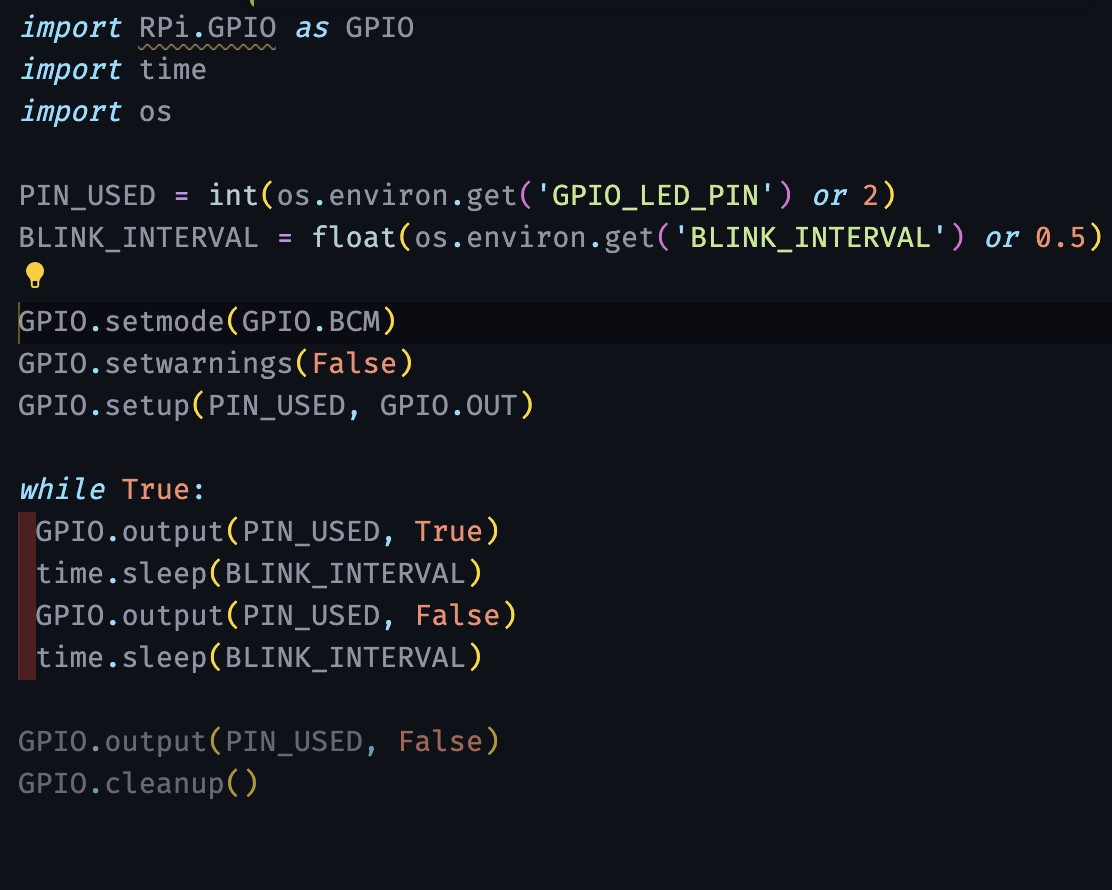
\includegraphics[width=0.8\textwidth]{resources/chapter-4/pengujian/pengujian-sistem-raspi-09-led.jpg}
    \caption{Python Raspi LED Script}
    \label{fig:raspi-python-led-script}
\end{figure}

Dari script tersebut, dibuat docker image dengan base image armv7 yang membungkus python tersebut agar dapat berjalan di sistem IoT. Docker image yang telah dibuat diunggah ke dockerhub dengan nama {gawrgare/led\textunderscore blink}. Isi dari dockerfile dapat dilihat pada lampiran \ref{fig:raspi-docker-led-script}. Setelah docker image tersedia, selanjutnya terdapat beberapa langkah yang harus disiapkan sebelum melakukan \textit{deployment} pada lingkungan raspberrypi.

\begin{enumerate}
    \item Membuat \textit{company} dengan nama "raspi-company" dan \textit{cluster\textunderscore name} "cluster-raspi". Hasil dapat dilihat pada lampiran \ref{fig:pengujian-sistem-raspi-01}
    \item Membuat user pada \textit{company} tersebut dengan email \textit{raspi@gmail.com}. Hasil dapat dilihat pada lampiran \ref{fig:pengujian-sistem-raspi-02}
    \item Login dengan kredensial yang telah dibuat
    \item Mengunjungi halaman /devices dan melakukan registrasi \textit{devices} untuk kedua RaspberryPi dengan daftar nama nodes yang dapat dilihat pada lampiran \ref{fig:pengujian-sistem-raspi-04}
          \begin{enumerate}
              \item \textit{Device} "raspi-master" untuk \textit{hostname masterpi} dengan nama \textit{cluster} yaitu "master-node-raspi"
              \item  \textit{Device} "raspi-worker" untuk \textit{hostname raspberrypi} dengan nama \textit{cluster} yaitu "worker-node-raspi"
          \end{enumerate}
    \item Mengunjungi halaman /groups dan membuat \textit{group} "raspi-group-blink". Hasil dapat dilihat pada lampiran \ref{fig:pengujian-sistem-raspi-05}
    \item Mengunjungi halaman group detail "raspi-group-blink" lalu menambahkan kedua device ke dalam group.
    \item Mengunjungi halaman \textit{deployment} lalu membuat repository dengan nama "raspi-image-blink" dan image\textit{ gawrgare/led\textunderscore blink}.
    \item Membuat deployment dengan nama "raspi-deployment-blink" dan mengisi target dengan "node=master" pada halaman \textit{deployment}.
\end{enumerate}

Layout dari RaspberryPi serta letak kabel dan LED dapat dilihat pada lampiran \ref{fig:pengujian-sistem-raspi-layout}. Setelah semua persiapan dilakukan, dilakukan pengujian dengan dua jenis \textit{deployment} yaitu \textit{target} dan \textit{custom} dengan versi \textit{group}.
\begin{enumerate}
    \item Target deployment merupakan deployment yang dilakukan sesuai dengan nilai target pada deployment object, dalam kasus ini target nya ialah node dengan attribut "node=master". Pengujian tipe ini hanya melakukan deployment dengan \textit{hostname masterpi} yang memiliki nama node "master-node-raspi". Setelah deployment dilakukan, LED yang terhubung dengan pin pada "master-node-raspi" berkedip, hal ini menunjukan bahwa proses deployment telah berhasil dilakukan. Hasil dapat dilihat pada lampiran \ref{fig:hasil-pengujian-sistem-raspi-target}.
    \item Custom deployment mengabaikan nilai target yang terdapat pada objek deployment dan melakukan deployment sesuai jenis serta id yang diinginkan. Terdapat dua jenis yaitu \textit{group} dan \textit{device}. Dalam kasus groups, Deployment dilakukan ke dua \textit{device} yang terhubung ke \textit{group} "raspi-group-blink". Setelah deployment dilakukan, kedua LED berkedip menunjukan bahwa script berhasil dijalankan untuk setiap \textit{device} yang terhubung pada group. Hasil dapat dilihat pada lampiran \ref{fig:hasil-pengujian-sistem-raspi-custom}.
\end{enumerate}

Setelah deployment berhasil dilakukan, pengujian dilanjutkan dengan mengunjungi halaman detail dari "raspi-deployment-blink" untuk melihat riwayat deployment. Hasil dapat dilhat pada lampiran \ref{fig:pengujian-sistem-raspi-10}. Dapat dilihat bahwa pengujian dengan ID P20 hingga P31 menunjukan hasil yang sesuai dengan kebutuhan fungsional yang telah didefinisikan. Seluruh rekap pengujian sistem ini dapat dilihat pada lampiran \ref{tab:pengujian-sistem-raspi}.
\subsubsection{Penguijan Deployment MQTT Client untuk Mengirim data Temperatur pada \textit{Clutser GCP}}

Pengujian ini mencakup pengujian dengan ID P32 hingga P39. Pada pengujian sistem ini, dilakukan proses \textit{remote deployment} MQTT pada \textit{cluster GCP} dengan cluster name "prod-cluster-example". Pengujian ini dilakukan untuk mensimulasikan node sebagai sebuah sensor temperatur yang akan mengirimkan data sensornya melalui mqtt client ke mqtt broker. Pengujian ini membuktikan  \textit{compatibility} dari sistem yang tidak terbatas pada IoT namun seluruh perangkat yang berbasis UNIX yang dapat menjalankan kubernetes. Proses \textit{remote deployment} dilakukan dengan menggunakan image gawrgare/mqtt-client yang telah dibuat dan di \textit{publish} pada \textit{dockerhub}. Script yang digunakan untuk membuat image docker dibuat dengan python serta akan mengirimkan data dalam interval 5 detik. \textit{Script} dapat dilihat pada gambar \ref{fig:pengujian-gcp-script-docker-images}

\begin{figure}[ht]
  \centering
  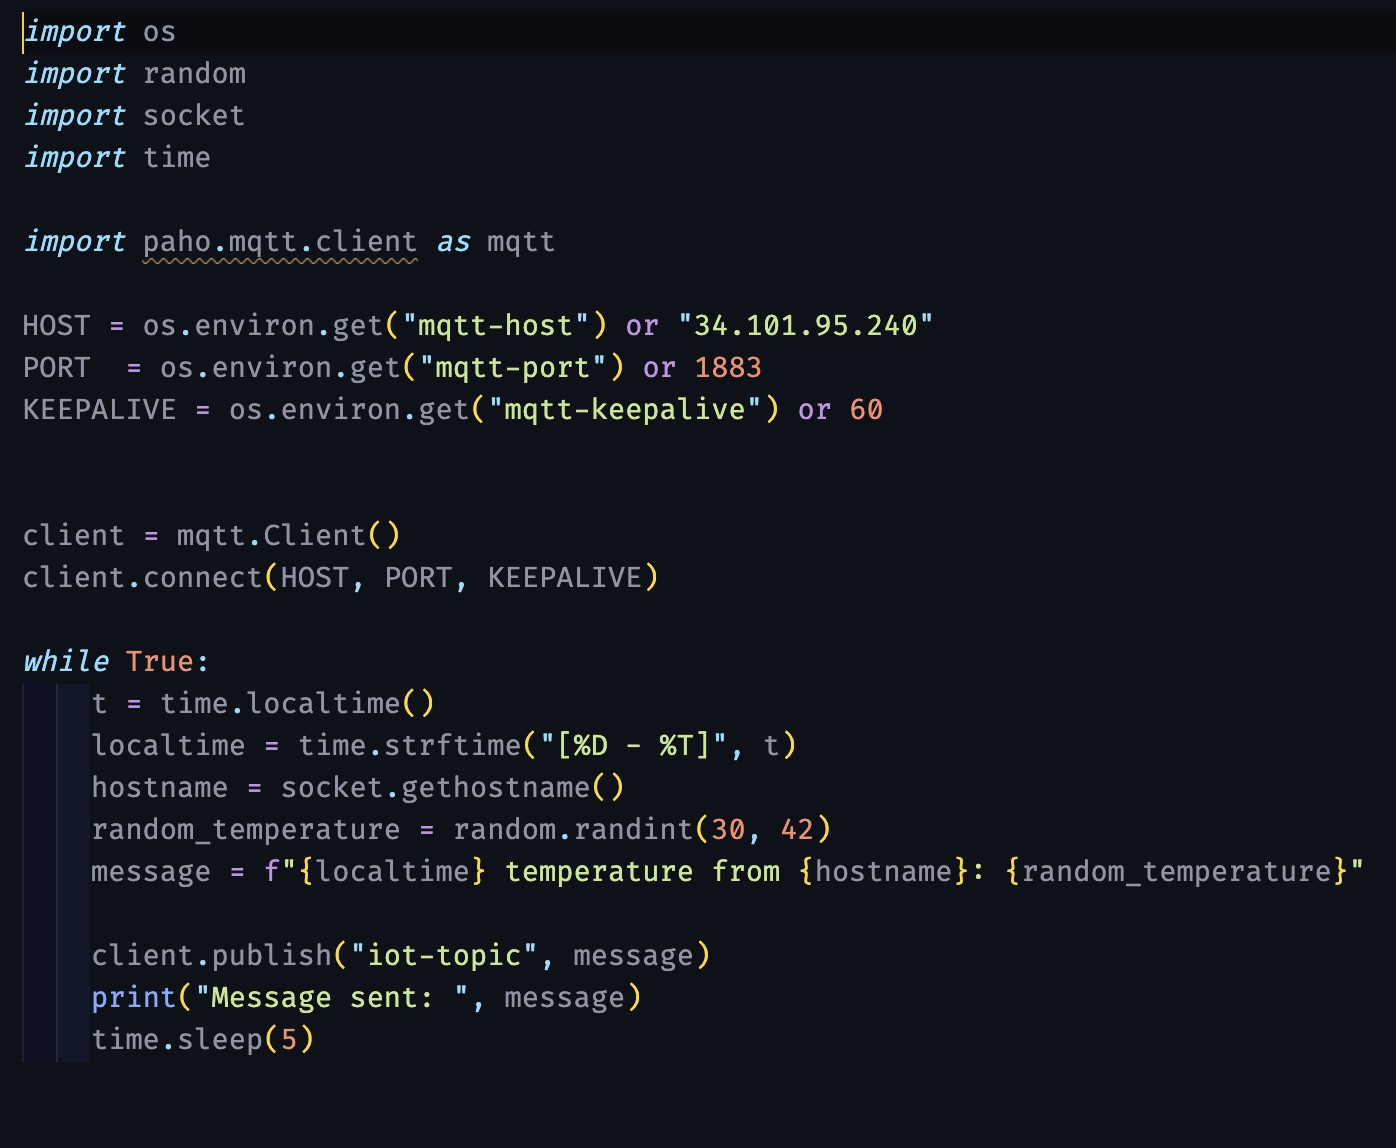
\includegraphics[width=0.8\textwidth]{resources/chapter-4/pengujian/pengujian-gcp-docker-image.jpg}
  \caption{Script MQTT Client untuk Docker Image gawrgare/mqtt-client}
  \label{fig:pengujian-gcp-script-docker-images}
\end{figure}

Pengujian dilakukan dengan mengikuti langkah langkah berikut:

\begin{enumerate}
  \item Melakukan setup mqtt-broker pada server yang memiliki IP 34.101.95.240.
  \item Membuat \textit{company} "test-semhas" dan nama cluster "prod-cluster-example". Hasil dapat dilihat pada lampiran \ref{fig:pengujian-sistem-gcp-01}
  \item Membuat \textit{user} dengan email "test@gmail.com", nama "test-user-semhas". Hasil dapat dilihat pada lampiran \ref{fig:pengujian-sistem-gcp-02}
  \item Login dengan menggunakan kredensial "test@gmail.com". Hasil dapat dilihat pada lampiran \ref{fig:pengujian-sistem-gcp-03}
  \item Mengunjungi halaman /devices lalu membuat \textit{device} "raspberrypi-pi-1" dan nama \textit{node} "master-cluster" serta memiliki label "sukses=aamiin". Hasil dapat dilihat pada lampiran \ref{fig:pengujian-sistem-gcp-04}
  \item Mengunjungi halaman /deployments lalu membuat \textit{deployment plan} untuk v1 dengan mengambil repository "gawrgare/mqtt-client" serta memiliki nama "mqtt-deployment". Hasil dapat dilihat pada lampiran \ref{fig:pengujian-sistem-gcp-05}
  \item Mengunjungi halaman /remote-deployment lalu melakukan \textit{deployment} dengan tipe "TARGET". Hasil dapat dilihat pada lampiran \ref{fig:pengujian-sistem-gcp-06}
  \item Setelah deployment berhasil dilakukan, hapus \textit{deployment} yang telah dibuat. Hasil dapat dilihat pada lampiran \ref{fig:pengujian-sistem-gcp-07}.
  \item Setelah deployment berhasil dibuat, jalankan kode untuk mengkonsumsi data dari mqtt-broker yang dikirimkan dari hasil deployment. Hasil dapat dilihat pada lampiran \ref{fig:pengujian-sistem-gcp-sukses-mqtt}
  \item Mengunjungi halaman /deployments lalu menghapus \textit{deployment plan} dengan nama "mqtt-deployment". Hasil dapat dilihat pada lampiran \ref{fig:pengujian-sistem-gcp-08}
  \item Mengunjungi halaman /deployments lalu menghapus \textit{deployment image} dengan nama "deploy-mqtt-client". Hasil dapat dilihat pada lampiran \ref{fig:pengujian-sistem-gcp-09}
\end{enumerate}

Setelah seluruh langkah dilakukan, pengujian dengan ID P32 hingga P39 berhasil diimplementasikan. Seluruh rekap pengujian dapat dilihat pada lampiran \ref{tab:pengujian-sistem-gcp}.

\subsubsection{Pengujian Gagal deployment}
Pengujian ini mencakup pengujian dengan ID40 hingga P46. Pada pengujian sistem ini, dilakukan proses \textit{Remote Deployment} yang gagal. Gagal berarti \textit{deployment} berhasil dilakukan dengan baik namun aplikasi gagal untuk dijalankan. Kegagalan dapat disebabkan oleh dua hal yaitu:
\begin{enumerate}
  \item Tidak ada \textit{device} yang memiliki label yang sesuai dengan target \textit{deployment}
  \item \textit{Image} yang tidak tersedia pada \textit{dockerhub}
\end{enumerate}
Pengujian ini akan mencakup kedua kegagalan yaitu dibuat \textit{deployment} dengan label yang tidak ada serta \textit{deployment} dengan image yang tidak ada pada \textit{dockerhub}. Ketika terjadi kegagalan proses \textit{deployment} akan secara otomatis dihapus karena terdapat sebuah \textit{asynchronus checking} setiap 10 detik dan sebuah timeout selama 200 detik yang membatasi waktu proses \textit{deployment}.

Pengujian kegagalan label dilakukan dengan mengikuti langkah langkah berikut:

\begin{enumerate}
  \item Login dengan menggunakan kredensial "test@gmail.com" dan password yaitu "inicontohpasswordges". Hasil dapat dilihat pada lampiran \ref{fig:pengujian-sistem-gagal-00}
  \item Mengunjungi halaman /deployments lalu buat \textit{deployment plan} dengan nama repository "deploy-mqtt-client" dengan v1 dan nama "deployment-plan-mqtt-client-failed" serta memiliki label "temperature=false". Hasil dapat dilihat pada lampiran \ref{fig:pengujian-sistem-gagal-01}
  \item Mengunjungi halaman /remote-deployment lalu melakukan \textit{deployment} dengan plan sebelumnya serta memiliki tipe "TARGET"
  \item \textit{Deployment} akan gagal karena tidak terdapat \textit{device} dengan label yang sesuai dengan \textit{deployment plan} Hasil dapat dilhat pada lampiran \ref{fig:pengujian-sistem-gagal-02}
  \item \textit{Program} akan melakukan \textit{polling} setiap 10 detik. Lalu setelah 200 detik \textit{deployment} akan dihapus, menandakan bahwa terdapat kegagalan pada \textit{deployment}. Hasil dapat dilhat pada lampiran \ref{fig:pengujian-sistem-gagal-03}
\end{enumerate}

Kegagalan pada kasus ini, disebabkan label pada deployment yang menargetkan "temperature=false" sedangkan kedua \textit{device} yang ada tidak memiliki label tersebut. Sehingga \textit{scheduler} pada kubernetes tidak bisa membuat \textit{deployment} dan sistem menghapus \textit{deployment} setelah melewati waktu \textit{timeout} 200 detik.

Selanjutnya, Pengujian kegagalan image dilakukan dengan mengikuti langkah langkah berikut:

\begin{enumerate}
  \item Login dengan menggunakan kredensial "test@gmail.com" dan password yaitu "inicontohpasswordges". Hasil dapat dilihat pada lampiran \ref{fig:pengujian-sistem-gagal-01}
  \item Mengunjungi halaman /deployments lalu membuat repository dengan image "nonexist-image". Hasil dapat dilihat pada lampiran \ref{fig:pengujian-sistem-gagal-06}
  \item Pada halaman yang sama, buat \textit{deployment plan} dengan repository yang telah dibuat dengan v1 dan nama "deployment-image" serta memiliki label "sukses=aamiin". Hasil dapat dilihat pada lampiran \ref{fig:pengujian-sistem-gagal-07}
  \item Mengunjungi halaman /remote-deployment lalu melakukan \textit{deployment} dengan plan sebelumnya serta memiliki tipe "TARGET"
  \item \textit{Deployment} akan gagal karena tidak menemukan image "nonexist-image" pada \textit{dockerhub}. Hasil dapat dilhat pada lampiran \ref{fig:pengujian-sistem-gagal-08}
  \item \textit{Program} akan melakukan \textit{polling} setiap 10s. Lalu setelah 200 detik \textit{deployment} akan dihapus, menandakan bahwa terdapat kegagalan pada \textit{deployment}. Hasil dapat dilhat pada lampiran \ref{fig:pengujian-sistem-gagal-09}
\end{enumerate}

Kegagalan pada pengujian ini disebabkan oleh tidak tersedianya image "nonexist-image" pada \textit{dockerhub}. Hal ini menyebabkan terjadi error ketika proses \textit{deployment} yaitu ErrImagePull, yang diakibatkan error ketika mengambil image dari \textit{dockerhub} seperti pada lampiran \ref{fig:pengujian-sistem-gagal-08}. Setelah seluruh rangkaian pengujian dilakukan, pengujian dengan ID P40 hingga P46 berjalan sesuai ekspektasi. Seluruh rekap pengujian ini dapat dilihat pada lampiran \ref{tab:pengujian-sistem-gagal}

\subsection{Pengujian Non Fungsional}
Pada bagian ini, dilakukan pengujian terhadap kebutuhan non-fungsional sistem. Terdapat dua kebutuhan non-fungsional yang akan diuji yaitu \textit{Security dan Portability}. Pengujian akan menggunakan \textit{security testing} dan \textit{compatibility testing} untuk masing masing kebutuhan non-fungsional.

\subsubsection{\textit{Security Testing}}
\textit{Security Testing} bertujuan untuk menguji kebutuhan non-fungsional yaitu \textit{security}. Pengujian ini hanya terbatas pada masalah autentikasi dan authorisasi. Pengujian kebutuhan non-fungsional ini dilakukan dengan cara mencoba mengakses \textit{dashboard} dan \textit{service} tanpa meletakan token yang valid. Pengujian ini mencakup ID pengujian P47 hingga P50

\begin{enumerate}
  \item Mengakses \textit{dashboard} tanpa kredensial

        Ketika mengakses \textit{dashboard} tanpa memiliki kredensial, \textit{dashboard} memiliki \textit{middleware} yang akan mengecek token yang disimpan pada \textit{client}. Jika token tidak valid maka sistem akan langsung melakukan \textit{redirect} ke halaman login.

  \item Mengakses user \textit{service} tanpa kredensial

        Ketika mencoba untuk mengakses \textit{service} pada endpoint apapun, \textit{service} memiliki \textit{middleware}
        yang akan mengecek header authentikasi yang dikirimkan oleh client. Jika kredensial pada header tidak dicantumkan maka akan mengembalikan \textit{401 Unauthorized} seperti pada lampiran \ref{fig:akses-service-user}.

  \item Mengakses admin \textit{service} tanpa kredensial

        Admin endpoint memiliki \textit{middleware} validateAdminJWTKey. Ketika mencoba untuk mengakses \textit{endpoint} admin tanpa memberikan header X-Admin-Api-Key yang sesuai maka \textit{service} akan mengembalikan \textit{401 Unauthorized} seperti pada lampiran \ref{fig:akses-service-admin}.

  \item Mengakses \textit{url kubernetes} tanpa kredensial

        Seluruh cluster kubernetes akan mengexpose endpoint pada port 6443. Pengujian ini akan mengakses url kubernetes yaitu https://34.101.95.240:6443/. Ketika diakses, hasilnya akan menunjukan status \textit{401 Unauthorized} seperti pada lampiran \ref{fig:akses-service-kubernetes}.

\end{enumerate}

Setelah melakukan pengujian, pengujian dengan ID P47 hingga P50 berjalan sesuai dengan ekspektasi yaitu menunjukan kegagalan saat mengakses \textit{resource} yang diminta. Seluruh rekap pengujian dapat dilihat pada tabel \ref{tab:pengujian-nonfungsional-security}.

\subsubsection{Compatibility Testing}
\textit{Compatibility testing} dilakukan untuk menguji kebutuhan non-fungsional yaitu \textit{portability}. Pengujian kebutuhan non-fungsional ini dialkukan dengan tiga skenario yaitu mengakses \textit{dashboard} dari mobile serta mengakses dari berbagai \textit{browser}. Tujuan dari pengujian ini adalah memastikan bahwa \textit{dashboard} dapat dijalankan pada berbagai \textit{platform}. Pengujian ini mencakup pengujian dengan ID P52 hingga P54.

\begin{enumerate}
  \item Mengakses \textit{dashboard} dari perangkat mobile

        \textit{Dashboard} berhasil diakses melalui perangkat mobile dan dapat dilihat hasil dapat dilihat pada lampiran \ref{fig:akses-dashboard-mobile}.

  \item Mengakses \textit{dashboard} dari Chromium based browser

        \textit{Dashboard} berhasil diakses melalui browser \textit{chromium based} yaitu "Arc" dan "Google Chrome" yang dapat dilhat pada lampiran \ref{fig:akses-dashboard-chromium}.

  \item Mengakses \textit{dashboard} dari browser safari

        \textit{Dashboard} berhasil diakses melalui browser safari yang dapat dilhat pada lampiran \ref{fig:akses-dashboard-safari}.

\end{enumerate}

Setelah melakukan pengujian, pengujian dengan ID P51 hingga P53 berjalan sesuai dengan ekspektasi yaitu menunjukan kegagalan saat mengakses \textit{resource} yang diminta. Seluruh rekap pengujian dapat dilihat pada tabel \ref{tab:pengujian-nonfungsional-compatibility}.
Berdasarkan \textit{security testing} dan \textit{compatibility testing}, sistem \textit{remote deployment} yang dibuat telah memenuhi kebutuhan non-fungsional yang telah di definisikan pada tabel kebutuhan yang dapat dilihat pada lampiran \ref{tab:kebutuhan-non-fungsional}
